\documentclass[submit]{harvardml}

% Put in your full name and email address.
\name{Weiyi Chen}
\email{wec427@g.harvard.edu}

% List any people you worked with.
\collaborators{%
N.A.
}

% You don't need to change these.
\course{CS181-S16}
\assignment{Assignment \#2}
\duedate{5:00pm February 26, 2016}

\usepackage[OT1]{fontenc}
\usepackage[colorlinks,citecolor=blue,urlcolor=blue]{hyperref}
\usepackage[pdftex]{graphicx}
\usepackage{subfig}
\usepackage{fullpage}
\usepackage{palatino}
\usepackage{mathpazo}
\usepackage{amsmath}
\usepackage{amssymb}
\usepackage{color}
\usepackage{todonotes}
\usepackage{listings}
\usepackage{common}
\usepackage{bm}

\usepackage[mmddyyyy,hhmmss]{datetime}

\definecolor{verbgray}{gray}{0.9}

\lstnewenvironment{csv}{%
  \lstset{backgroundcolor=\color{verbgray},
  frame=single,
  framerule=0pt,
  basicstyle=\ttfamily,
  columns=fullflexible}}{}

\begin{document}
\begin{center}
{\Large Homework 2: Linear Classification}\\
\end{center}

There is a mathematical component and a programming
component to this homework. Please submit your PDF to Canvas, and push everything in Github.

This homework is about multi-class classification. Whereas in more simple
classification models we build classifiers that discriminate between two classes,
in multi-class regression, we discriminate between three or more classes.  As
usual, we imagine that we have the input matrix $\boldX \in \reals^{N \times D}$
(or perhaps they have been mapped to some basis $\bm{\Phi}$, without loss
of generality) but that our outputs are now ``one-hot coded''.  What that means
is that, if there are~$K$ output classes, rather than representing the output
labels as integers~${1,2,\ldots,K}$, we represent them as a binary vectors of
length~$K$.  These vectors are zero in each component except for the one
corresponding to the correct label, and that entry has a one.  So, if there are
7 classes and a particular datum has label 3, then the target vector would
be~${[0,0,1,0,0,0,0]}$ (assuming the labels are 1-indexed).

In the first problem, you will be exploring the properties of the softmax
function, which is central to multiclass logistic regression.  In the second
problem, we will have you dive into the matrix algebra and methods behind
generative classifications.  Finally, in the third problem, you will implement a
generative classifier and logistic regression from close to scratch, and the
first two problems should inform this!

%\subsection*{1. Properties of Softmax [5pts]}
%%%%%%%%%%%%%%%%%%%%%%%%%%%%%%%%%%%%%%%%%%%%%
% Problem 1
%%%%%%%%%%%%%%%%%%%%%%%%%%%%%%%%%%%%%%%%%%%%%
\begin{problem}[Properties of Softmax , 5pts]

Logistic regression is a discriminative probabilistic model: a prediction
consists of a distribution over the different classes. In other words, logistic
regression outputs a vector of nonnegative numbers that sum to one.

The softmax function generalizes the logistic sigmoid to the case of $K$
classes: it takes as input a vector, and outputs a K dimensional vector in the
range $[0,1]$ whose components sum to $1$:

\[ \bm{\sigma}(\mathbf{z}) = softmax(\mathbf{z}) =
\frac{\exp(\mathbf{z})}{\sum_i\exp(z_i)}\]

In logistic regression, we often use the softmax-based parameterization over $K$ vectors $\{\boldw_k\}$:

\begin{align*}
  \Pr(t_{nk}=1 \given \boldX, \{\boldw_{k'}\}^K_{k'=1})
  &= \frac{ \exp\{ \boldw_k^{\trans}\boldx_n \} }
  { \sum_{k'=1}^K \exp\{ \boldw_{k'}^{\trans}\boldx_n \} }\,.
\end{align*}

Here we're using~${t_{nk}=1}$ to indicate the probability that the $n$th entry
is assigned to the $k$th class.\\

Softmax is a crucial function in logistic regression, and you will see it again in other models, such as neural networks. 
So, we want you to start gaining the intuitions for the properties of softmax, and for common methods that employ it. 

Show that:
\begin{enumerate}
  \item The output of the softmax function is always a vector with non-negative components
    that are at most 1. 
  \item The output of the softmax function forms a distribution (the components sum to 1).
  \item Softmax preserves order. This means that if the elements of $\mathbf{z}$ have some order, then the elements of $\bm{\sigma}(\mathbf{z})$ have the same order. 
  \item Equation 4.106 from Bishop holds
  \item Using your answer to the previous question, show that equation 4.109
    holds. By the way, this may be useful for Problem 3!
\end{enumerate}
\end{problem}
\subsection*{Solution}

\begin{enumerate}
    \item The $k$-th component of the output vector of the softmax function is 
    $$ \frac{\exp(z_k)}{\sum_i\exp(z_i)} > 0, \forall k $$
    which is non-negative because $exp(x) > 0, \forall x \in \mathcal{R}$.
    Since every component is non-negative, then
    $$ \exp(z_k) \le \exp(z_k) + \sum_{i\neq k} \exp(z_i) \le \sum_{i} \exp(z_i) $$
    therefore 
    $$ \frac{\exp(z_k)}{\sum_i\exp(z_i)} \le 1, \forall k $$
    The output of the softmax function is always a vector with non-negative components that are at most $1$.
    \item The output of the softmax function forms a distribution because the components sum to $1$, 
    $$ \sum_k \frac{\exp(z_k)}{\sum_i\exp(z_i)} = \frac{\sum_k\exp(z_k)}{\sum_i\exp(z_i)} = 1 $$
    \item For any two elements of $\boldz$ with index $j$ and $k$, assume without loss of generality that $z_j \ge z_k$, then according to the property that the exponential is a monotonically increasing continuous function, then
    $$ \exp(z_j) \ge \exp(z_k) $$
    Therefore it does not change the order of any two elements, i.e. 
    $$ \frac{\exp(z_j)}{\sum_i\exp(z_i)} \ge \frac{\exp(z_k)}{\sum_i\exp(z_i)}, \forall j, k \text{ such that } z_j \ge z_k $$
    Softmax preserves order.
    \item This is to show the derivatives of the softmax activation function (4.104), which is equivalent to the notation above, 
    $$ p(\mathcal{C}_k \given \phi) = y_k(\phi) = \frac{\exp(a_k)}{\sum_j \exp(a_j)} $$
    where the $a_k$ are defined by (4.105), 
    $$ a_k = \boldw_k^T \phi $$
    are given by (4.106),
    $$ \frac{\partial y_k}{\partial a_j} = y_k(I_{kj} - y_j) $$
    
    If $j = k$, from (4.104) we have
    $$ \frac{\partial y_k}{\partial a_k} = \frac{e^{a_k}}{\sum_i e^{a_i}} - \left(\frac{e^{a_k}}{\sum_i e^{a_i}} \right)^2 = y_k(1-y_k) $$
    If $j \neq k$, from (4.104) we have
    $$ \frac{\partial y_k}{\partial a_j} = -\frac{e^{a_k}e^{a_j}}{\left(\sum_i e^{a_i}\right)^2} = -y_ky_j $$
    Combining these two we derive (4.106) for any $j, k$,
    $$ \frac{\partial y_k}{\partial a_j} = y_k(I_{kj} - y_j) $$
    \item We start by computing the derivative of (4.108) w.r.t. $y_{nk}$
    $$ \frac{\partial E}{\partial y_{nk}} = -\sum_{k=1}^{K}\frac{t_{nk}}{y_{nk}} $$
    From (4.106), we see that
    $$ \frac{\partial y_{nk}}{\partial a_{nj}} = y_{nk}(I_{kj} - y_{nj}) $$
    Finally, we have
    $$ \nabla_{\boldw_j} a_{nj} = \phi_n $$
    where $\nabla$ denotes the gradient with respect to w. Combining these three using the chain rule, we obtain
    $$ \nabla_{\boldw_j} E = \sum_{n=1}^N \frac{\partial E}{\partial y_{nk}} \cdot \frac{\partial y_{nk}}{\partial a_{nj}} \cdot \nabla_{\boldw_j} a_{nj} = \sum_{n=1}^{N} \sum_{k=1}^K t_{nk}(y_{nj} - I_{kj}) \phi_n $$
    Note that according to the answer of part 2, 
    $$ \sum_{k=1}^K t_{nk}y_{nj} = y_{nj} $$  
    and 
    $$ \sum_{k=1}^K t_{nk}I_{kj} = t_{nj} $$ 
    Therefore
    $$ \nabla_{\boldw_j} E = \sum_{n=1}^{N} (y_{nj} - t_{nj}) \phi_n $$
\end{enumerate}

%\subsection*{2. Mooooar matrix calculus [10 pts]}
%%%%%%%%%%%%%%%%%%%%%%%%%%%%%%%%%%%%%%%%%%%%%
% Problem 2
%%%%%%%%%%%%%%%%%%%%%%%%%%%%%%%%%%%%%%%%%%%%%
\begin{problem}[Mooooar matrix calculus , 10pts]
\textbf{Note - this problem appears longer than it is, since we broke up one problem into separate parts rather
than having you do all of these steps at once. Many of these subparts may be just one or two lines.}\\

Consider a generative K-class model.  We define the class prior with vector
$\vec \pi$: $\mathbb{P}(\mathcal{C}_k) = \pi_k$.  We define the
class-conditional densities $\mathbb{P}(\phi|\mathcal{C}_k)$ where $\phi$ is the
input feature vector. Consider the data set $\{\phi_n, {\bf t}_n\}$ where $n = 1 \dots N$ where ${\bf
t}_n \in \{0,1\}^K$ is a one-hot encoded target vector. This means that
$\bf{t}_n$ is 0 everywhere, except for in the $k$th position, where $k$ is the
class assigned to the $n$th feature vector.
\begin{enumerate}
  \item Write out the complete-data log-likelihood of the data set using only the
    notations introduced in the problem formulation above.
    $$\ln \mathbb{P}(\{\phi_n, {\bf t}_n \} | \{\pi_k \}) =?$$
  \item Since the prior forms a distribution, it has the constraint that
    $\sum_k\pi_k - 1 = 0$.  Using the hint at the end of the exercise, give the
    expression for the maximum-likelihood estimator for the prior
    class-membership probabilities:
    $$\hat \pi_k =?$$
    Make sure to write out the intermediary equation you need
    to solve to obtain this estimator. Double-check your answer: the final
    result should be very intuitive!
\end{enumerate}
    We will suppose for the remaining questions of this exercise that the
    class-conditional probabilities are given by gaussian distributions with the
    same covariance matrix:
    $$\mathbb{P}(\phi | C_k) = \mathcal{N}(\phi | \vec \mu_k, \Sigma)$$
    \begin{enumerate}
  \item[3.] Write out the gradient of log-likelihood with respect to vector $\mu_k$.
    Write the expression in matrix form as a function of the variables defined
    throughout this exercise. Simplify as much as possible for full credit.
  \item[4.] Write out the maximum-likelihood estimator for vector $\mu_k$. Once
    again, your final answer should seem intuitive.
  \item[5.] Write out the gradient for the log-likelihood with respect to the
    covariance matrix $\Sigma$. Even though the log-likelihood function is a
    scalar function, since you are differentiating with respect to a
    \emph{matrix}, the resulting expression should be a matrix!
  \item[6.] Express the maximum likelihood estimator of the covariance matrix.
\end{enumerate}

\paragraph{Hint.} When maximizing a function $f$ with respect to an equality
constraint that needs to be met at the optimum (which can always be written as
$g(x) = 0$), we introduce a Lagrange multiplier $\lambda$ and maximize: $$\max_x
f(x) + \lambda g(x)$$

\paragraph{Cookbook formulas.} Here are some formulas you might want to consider
using to compute difficult gradients. You can use them as is in the homework
without proof. If you are looking to hone your matrix calculus skills, try to
find different ways to prove these formulas yourself (will not be part of the
evaluation of this homework). In general, you can use any formula from the matrix cookbook,
as long as you cite it. We opt for the following common notation:
$X^{-T} := (X^{-1})^{-T} = (X^{T})^{-1}$
\begin{align*}
  & \frac{\partial a^T X^{-1} b}{\partial X} = - X^{-T} a b^T X^{-T} \\
  & \frac{\partial \ln | \det (X) |}{\partial X} = X^{-T}
 \end{align*}
 \end{problem}


\subsection*{Solution}
\begin{enumerate}
    \item The probability of one data point is
    $$ P(\phi, \boldt) = P(\phi \given \boldt) P(\boldt) = \prod_{k=1}^K (P(\phi \given C_k) \pi_k)^{\boldt_k} $$
    I denote the parameters of this model as $\theta$. The independent samples allow us to take a product over the data points.
    $$ \mathcal{L}(\theta) = \prod_{n=1}^{N}\prod_{k=1}^K (P(\phi_n \given C_k) \pi_k)^{t_{nk}} $$
    Thus,
    $$ l(\theta) = \sum_{n=1}^{N} \sum_{k=1}^K t_{nk} [\log(P(\phi_n \given C_k)) + \log\pi_k] $$
    
    \item We want to maximize the log likelihood subject to the constraint that $\sum_k\pi_k - 1 = 0$. Thus, we must introduce Lagrange Multipliers. The parameters we care about here are the $\pi_k$'s. Here is the Lagrangian:
    $$ \mathcal(\pi, \lambda) = \sum_{n=1}^{N} \sum_{k=1}^K t_{nk} [\log(P(\phi_n \given C_k)) + \log\pi_k] + \lambda(\sum_{k=1}^K\pi_k - 1) $$
    Taking the derivative with respect to $\pi_k$ and setting it to 0, we have
    $$ \frac{\partial}{\partial \pi_k} \mathcal{L}(\pi, \lambda) = \frac{1}{\pi_k} \sum_{n=1}^N t_{nk} + \lambda = 0 \Rightarrow \pi_k = -\frac{1}{\lambda} \sum_{n=1}^N t_{nk} = -\frac{N_k}{\lambda} $$
    where $N_k$ is the number of data points whose label is class $k$. Taking the derivative with respect to $\lambda$, we have
    $$ \frac{\partial}{\partial \lambda} \mathcal{L}(\pi,\lambda) = \sum_{k=1}^K \pi_k - 1 = 0 \Rightarrow \sum_{k=1}^K \pi_k = 1 $$
    We can plug in all of our values of the $\pi_k$'s into the constraint, giving us the value of $\lambda$:
    $$ \sum_{k=1}^K \pi_k = \sum_{k=1}^K - \frac{N_k}{\lambda} = -\frac{N}{\lambda} = 1 \Rightarrow \lambda = -N $$
    After having solved for $\lambda$, we can just plug this back into our other equations to solve for our $\pi_k$'s. Thus, we have that the maximum likelihood estimates of the prior probabilities are
    $$ \pi_k = \frac{N_k}{N} $$
    
    \item The gradient of log-likelihood with respect to vector $\mu_k$ is 
    $$ \frac{\partial l(\theta)}{\partial \mu_k} = \sum_{n=1}^{N} t_{nk} \frac{\partial \log(P(\phi_n \given C_k))}{\partial \mu_k} $$
    Since we are given $\mathbb{P}(\phi | C_k) = \mathcal{N}(\phi | \vec \mu_k, \Sigma)$, recall that
    $$ \mathcal{N}(\phi \given \mu_k, \Sigma) = \frac{1}{\sqrt{(2\pi)^k|\Sigma|}}  \exp\left(-\frac{1}{2} (\phi - \mu_k)^{\rm T} \Sigma^{-1} (\phi-\mu_k)\right) $$
    Then 
    $$ \frac{\partial P(\phi_n \given C_k)}{\partial \mu_k} = -\frac{1}{2} \left( \frac{\partial(\phi_n - \mu_k)^T\Sigma^T(\phi_n - \mu_k)}{\partial\mu_k} \right) = -\frac{1}{2} (-2\Sigma^T(\phi_n-\mu_k)) = \Sigma^T(\phi_n-\mu_k) $$ 
    Plug in the first formula, we have
    $$ \frac{\partial l(\theta)}{\partial \mu_k} = \sum_{n=1}^N t_{nk} \Sigma^T(\phi_n-\mu_k) = - N_k\Sigma^T\mu_k + \sum_{n=1}^N t_{nk}\Sigma^T\phi_n  $$
    where we used the notation that $ N_k = \sum_{n=1}^N t_{nk} $.
    
    \item Let the gradient of last part be zero, we have
    $$ - N_k\Sigma^T\mu_k + \sum_{n=1}^N t_{nk}\Sigma^T\phi_n = 0 \Rightarrow \mu_k = \frac{1}{N_k} \sum_{n=1}^N t_{nk}\phi_n $$
    
    \item The gradient of log-likelihood with respect to vector $\mu_k$ is 
    $$ \frac{\partial l(\theta)}{\partial \Sigma} = \sum_{n=1}^{N} \sum_{k=1}^K t_{nk} \frac{\partial \log(P(\phi_n \given C_k))}{\partial \Sigma} $$
    then 
    $$ \frac{\partial P(\phi_n \given C_k)}{\partial \Sigma} = -\frac{1}{2} (\frac{\partial\ln|\det(\Sigma)|}{\partial\Sigma} + \frac{\partial(\phi_n - \mu_k)^T\Sigma^T(\phi_n - \mu_k)}{\partial\Sigma}) = -\frac{1}{2} (\Sigma^{-1} - \Sigma^{-1}(\phi_n - \mu_k)(\phi_n - \mu_k)^T\Sigma^{-1}) $$
    Plug in the first formula, we have
    $$ \frac{\partial l(\theta)}{\partial \Sigma} = -\sum_{n=1}^{N} \sum_{k=1}^K \frac{t_{nk}}{2} (\Sigma^{-1} - \Sigma^{-1}(\phi_n - \mu_k)(\phi_n - \mu_k)^T\Sigma^{-1}) $$ 
    Using the fact that $ N_k = \sum_{n=1}^N t_{nk} $ and $\sum_k N_k = N$, we have
    $$ \frac{\partial l(\theta)}{\partial \Sigma} = -\frac{N}{2}\Sigma^{-1} + \sum_{n=1}^{N} \sum_{k=1}^K \frac{t_{nk}}{2}\Sigma^{-1}(\phi_n - \mu_k)(\phi_n - \mu_k)^T\Sigma^{-1} $$ 
    
    \item Let the gradient of last part be zero, we have
    $$ -\frac{N}{2}\Sigma^{-1} + \sum_{n=1}^{N} \sum_{k=1}^K \frac{t_{nk}}{2}\Sigma^{-1}(\phi_n - \mu_k)(\phi_n - \mu_k)^T\Sigma^{-1} = 0 $$
    then 
    $$ \Sigma = \frac{1}{N} \sum_{k=1}^K \sum_{n=1}^N t_{nk} (\phi_n - \mu_k)(\phi_n - \mu_k)^T $$
    if we assume 
    $$ \boldS_k = \frac{1}{N_k} \sum_{n=1}^N t_{nk} (\phi_n - \mu_k)(\phi_n - \mu_k)^T $$
    then
    $$ \Sigma = \sum_{k=1}^K \frac{N_k}{N} \boldS_k $$
\end{enumerate}


\newpage
\subsection*{3. Classifying Fruit [15pts]}
You're tasked with  classifying three different kinds of fruit, based on their
heights and widths.  Figure~\ref{fig:fruit} is a plot of the data.  Iain Murray
collected these data and you can read more about this on his website at
\url{http://homepages.inf.ed.ac.uk/imurray2/teaching/oranges_and_lemons/}.  We
have made a slightly simplified (collapsing the subcategories together) version
of this available as \verb|fruit.csv|, which you will find in the Github repository.
The file has three columns: type (1=apple, 2=orange, 3=lemon), width,
and height.  The first few lines look like this:
\begin{csv}
fruit,width,height
1,8.4,7.3
1,8,6.8
1,7.4,7.2
1,7.1,7.8
...
\end{csv}
\begin{figure}[h]
\centering
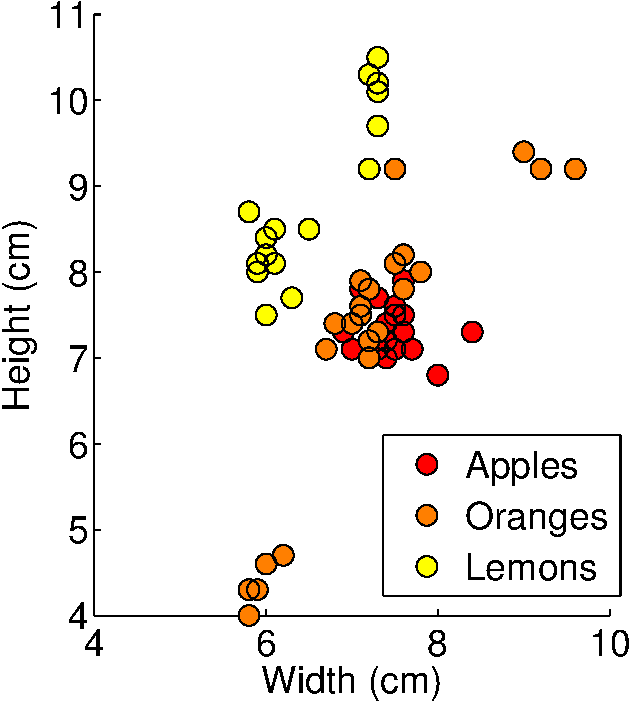
\includegraphics[width=0.5\textwidth]{fruit}
\caption{Heights and widths of apples, oranges, and lemons.  These fruit were
purchased and measured by Iain Murray:
\url{http://homepages.inf.ed.ac.uk/imurray2/teaching/oranges_and_lemons/}.}
\label{fig:fruit}
\end{figure}
\begin{problem}[Classifying Fruit, 15pts]
Please implement the following:
\begin{itemize}
\item Implement the three-class generalization of logistic regression, also
  known as softmax regression, for these data. You will do this by implementing
  gradient descent on the log likelihood. 
\item After this, implement a simple generative classifier with Gaussian
  class-conditional densities, as in Bishop Section 4.2.2. In particular, make
  two implementations of this, one with a shared covariance matrix across all of
  the classes, and one with a separate covariance being learned for each class.
  Note that the staff implementation can switch between these two by the
  addition of just a few lines of code. The shared covariance matrix case is
  detailed in Bishop (and you worked on it in Problem 2), and the separate covariance 
  case is only slightly different. In the separate covariance matrix case, the MLE for the
  covariance matrix of each class is simply the covariance of the data points assigned to that
  class, without combining them as in the shared case.
\end{itemize}
You may use anything in  numpy or scipy, except for scipy.optimize. That being said, if you happen to find a function in numpy or scipy that seems like it is doing too much for you, run it by a staff member. In general, linear algebra and random variable functions are fine. The controller file is problem3.py, in which you will specify parameters. The actual implementations you will write will be in LogisticRegression.py and GaussianGenerativeModel.py.


You will be given unimplemented class interfaces for GaussianGenerativeModel and LogisticRegression in the distribution code, 
and the code will indicate certain lines that you should not change in your final submission. Naturally, don't change these.
These classes will allow the final submissions to have consistency. There will also be a few hyperparameters that are set to
irrelevant values at the moment. You may need to modify these to get your methods to work.
The classes you implement follow the same pattern as scikit-learn, so they should be familiar to you. The distribution code currently outputs nonsense predictions just to show what the high-level interface should be, so you should completely remove the given predict() implementations and replace them with your implementations.

\begin{itemize}
\item The visualize() method for each classifier will save a plot that will show the decision boundaries. Please include those in this assignment.
\item Which classifiers model the distributions well? 
\item What explains the differences?
\end{itemize}
\end{problem}

\subsection*{Solution}

The three-class generalization of logistic regression and Gaussian generative classifiers with either shared or separate covariance are implemented in LogisticRegression.py and GaussianGenerativeModel.py respectively.

Below are the three plots

\begin{figure}[h]
    \centering
    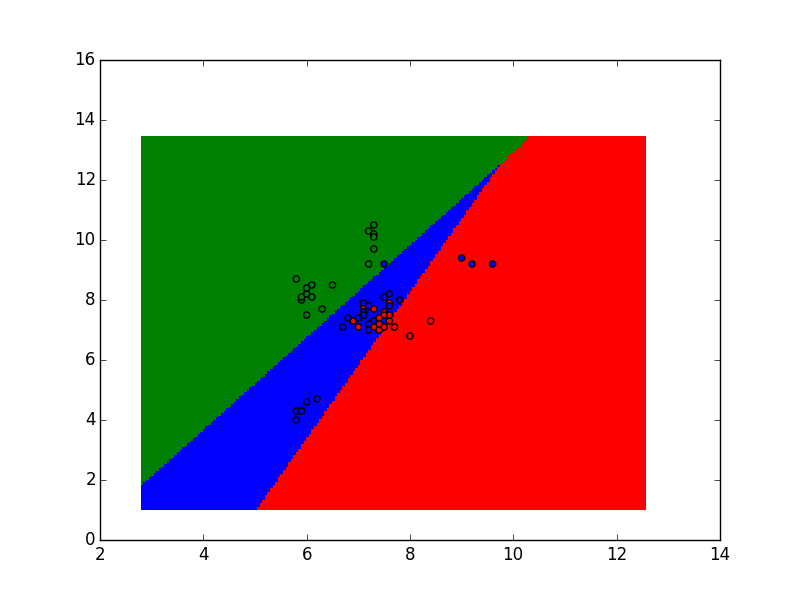
\includegraphics[width=400pt]{logistic_regression_result}
    \caption{Logistic Regression result}
\end{figure}

\begin{figure}[h]
    \centering
    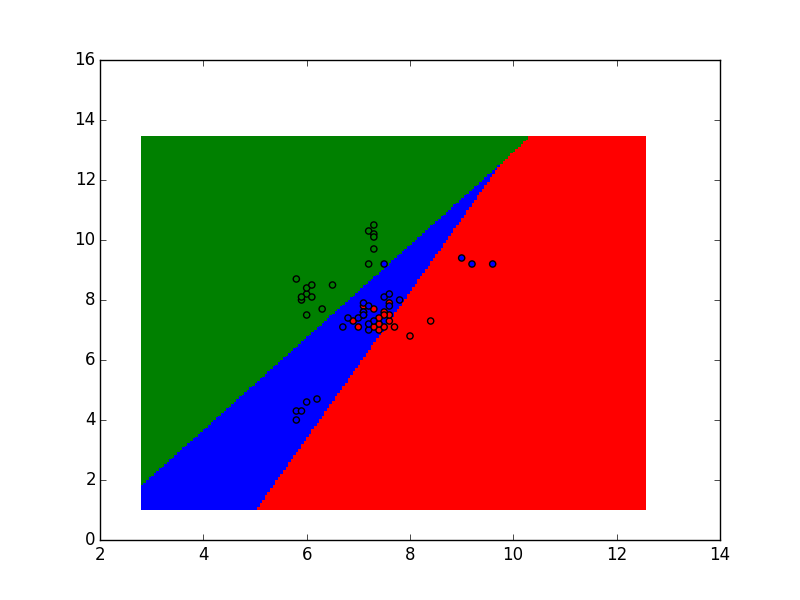
\includegraphics[width=400pt]{generative_result_separate_covariances}
    \caption{Generative result - separate covariances}
\end{figure}

\begin{figure}[h]
    \centering
    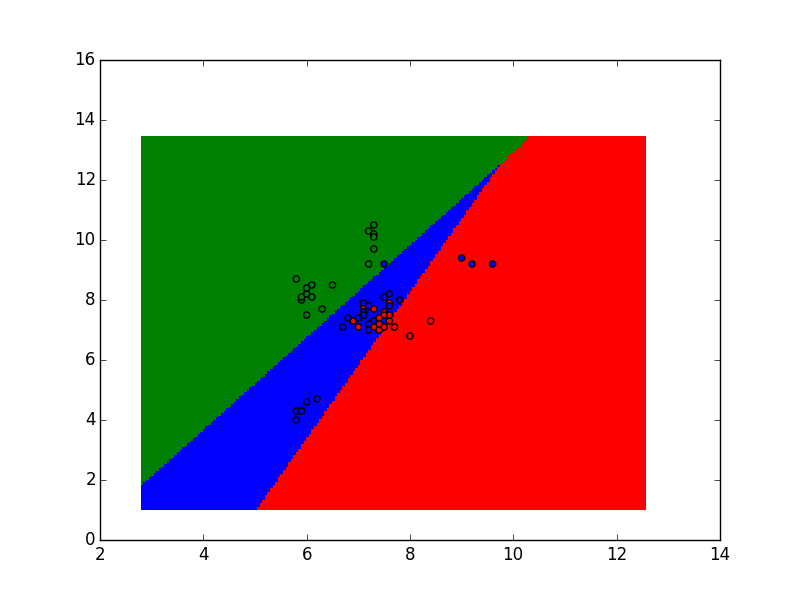
\includegraphics[width=400pt]{generative_result_shared_covariances}
    \caption{Generative result - shared covariances}
\end{figure}

\begin{itemize}
\item Which classifiers model the distributions well? 
\item What explains the differences?
\end{itemize}

It's hard to say which classifier is better, each one has its own benefits and shortcomings. Roughly speaking, I think Gaussian generative is better than Logistic regression.

In Logistic regression, it distinguishes green and others very well, however it's unable to separate red and blue, therefore all blue points are predicted incorrectly as red.

In Generative result - separate covariances, it distinguishes green from others very well (but not as perfect as logistic), also it predicts most of the blue points correctly though there are 3 blue points are recognized in red area. The shortcoming is that it's unable to predict most of the red points correctly since most of them are in blue area, but I believe this is good enough for linear barrier since there's a mixture between blue and red there.

In Generative result - shared covariances, the analysis on this image is similar to the separate one. It distinguishes green from others very well, and predicts most of the blue points correctly though there are 3 blue points are recognized in red area. The shortcoming is that it's unable to predict most of the red points correctly since most of them are in blue area. The difference of this one compared to the separate one is the margin of those incorrect-predicted red points, the margin of incorrect-predicted red points are larger while the margin of incorrect-predicted blue points are smaller in this plot.

All these three explain difference between green and the others, but only Gaussian Generative, either separate or shared, partially explains the difference between blue and red.

\newpage
\subsection*{Calibration [1pt]}
Approximately how long did this homework take you to complete?

\subsection*{Solution}
It took me almost 12 hours to complete.

\end{document}
